\documentclass[12pt]{article}
\usepackage[top=1in,left=1in, right = 1in, footskip=1in]{geometry}

\usepackage{graphicx}
%\usepackage{adjustbox}

\newcommand{\eref}[1]{(\ref{eq:#1})}
\newcommand{\fref}[1]{Fig.~\ref{fig:#1}}
\newcommand{\Fref}[1]{Fig.~\ref{fig:#1}}
\newcommand{\sref}[1]{Sec.~\ref{#1}}
\newcommand{\frange}[2]{Fig.~\ref{fig:#1}--\ref{fig:#2}}
\newcommand{\tref}[1]{Table~\ref{tab:#1}}
\newcommand{\tlab}[1]{\label{tab:#1}}
\newcommand{\seminar}{SE\mbox{$^m$}I\mbox{$^n$}R}

\usepackage{amsthm}
\usepackage{amsmath}
\usepackage{amssymb}
\usepackage{amsfonts}

%\usepackage{lineno}
%\linenumbers

\usepackage[pdfencoding=auto, psdextra]{hyperref}

\usepackage{natbib}
\bibliographystyle{chicago}
\date{\today}

\usepackage{xspace}
\newcommand*{\ie}{i.e.\@\xspace}

\usepackage{color}

\newcommand{\Rx}[1]{\ensuremath{{\mathcal R}_{#1}}} 
\newcommand{\Ro}{\Rx{0}}
\newcommand{\RR}{\ensuremath{{\mathcal R}}}
\newcommand{\Rhat}{\ensuremath{{\hat\RR}}}
\newcommand{\tsub}[2]{#1_{{\textrm{\tiny #2}}}}

\newcommand{\comment}[3]{\textcolor{#1}{\textbf{[#2: }\textsl{#3}\textbf{]}}}

%% \newcommand{\rev}[1]{\comment{red}{REV}{#1}}
\newcommand{\rev}[1]{}

\newcommand{\swp}[1]{\comment{magenta}{SWP}{#1}}
\newcommand{\jd}[1]{\comment{magenta}{JD}{#1}}
\newcommand{\new}[1]{\textcolor{blue}{#1}}

\begin{document}

\begin{flushleft}{
	\Large
	\textbf\newline{
		Evaluating uncertainties associated with preliminary estimates of the basic reproductive number during the novel coronavirus (2019-nCoV) outbreak
	}
}

\bigskip

% *swp2@princeton.edu
\end{flushleft}

\section*{Abstract}

\pagebreak

\section{Introduction}

Since December 2019, the novel coronavirus (2019-nCoV) has been spreading in China and other parts of the world.
As of January 28th, 2020, the World Health Organization has confirmed 4593 cases, including 56 confirmed cases in 14 different countries, outside China \citep{who28report}.
Although the virus is believed to have originated from animal reservoirs \citep{cdcncov}, 
there is clear evidence that it can be directly tranmitted between humans,
posing a greater threat for its spread.
\jd{It is spread primarily from person to person; that's been obvious for a while and is now confirmed. We should find a better cite and leave Viet Nam out of it.}

As the disease continues to spread, many researchers have published analyses of the outbreak, many focusing in particular on estimates of the basic reproductive number $\mathcal R_0$ (i.e., the average number of secondary cases generated by a primary case in a fully susceptible population \citep{anderson1991infectious, diekmann1990definition}).
Estimating the basic reproductive number is of interest during an outbreak because it provides information about the level of intervention required to interrupt transmission \citep{anderson1991infectious}, and about the final size of the outbreak \citep{anderson1991infectious, ma2006generality}.
However, it can be difficult to assess the validity of the estimates of $\mathcal R_0$ (as well as the associated degrees of uncertainty) when the estimation methods and their underlying assumptions vary widely, especially since these assumptions can directly affect the estimates.

Here, we show that a wide range of approaches to estimating \Ro\ present a simple framework for evaluating uncertainties 
associated with the estimates of $\mathcal R_0$
across a wide range of models using a generation-interval based approach and compare early estimates of $\mathcal R_0$ of the 2019-nCoV outbreak.
Our results indicate that most early estimates of $\mathcal R_0$ for the outbreak
are likely to have been overly confident.

\section{Methods}

Early in an outbreak, $\mathcal R_0$ cannot be estimated directly;
instead, $\mathcal R_0$ is often inferred from
the exponential growth rate $r$, which can be estimated reliably from incidence data \citep{mills2004transmissibility, nishiura2009transmission, ma2014estimating}. 
Given an estimate of the exponential growth rate $r$ and a distribution $g(\tau)$ of
generation intervals (i.e., the time between when a person become 
infected and that person infects another person \citep{svensson2007note}), the basic reproductive
number can be estimated via the Euler-Lotka equation \citep{wallinga2007generation}:
\begin{equation}
1/\mathcal R_0 = \int \exp(-r\tau) g(\tau) d\tau.
\end{equation}
In other words, estimates of $\mathcal R_0$ must
depend on the assumptions about the
exponential growth rate $r$ and the shape of the generation-interval distribution $g(\tau)$.

Here, we use the gamma approximation framework \citep{park2019practical} to (1) characterize the amount of uncertainty present in the exponential growth rates and the shape of the generation-interval distribution and (2) assess the degree to which these uncertainties affect the estimate of $\mathcal R_0$.
\jd{We should cite another group as well about this approximation.}
Assuming that generation intervals follow a gamma distribution
with the mean $\bar G$ and the squared coefficient of variation (CV$^2$) $\kappa$, 
we have
\begin{equation}
\mathcal R_0 = \left(1 + \kappa r \bar{G}\right)^{1/\kappa}.
\label{eq:gamma}
\end{equation}
This equation demonstrates that a generation-interval distribution
that has a larger mean (higher $\bar{G}$) or is less variable (lower $\kappa$)
will give a higher estimate of $\mathcal R_0$ for the same value of $r$.

\begin{table}[t]
\begin{center}
\footnotesize
\begin{tabular}{l|l|l|l}
 & Basic reproductive number & mean generation time (days) & CV$^2$ generation time \\
\hline
Study 1 & 2.5 (1.5--3.5)$^\ast$ & 8.4 & unspecified$^\dagger$ \\
\hline
Study 2 & 2.92 (95\% CI: 2.28--3.67) & 8.4 & 0.2 \\
\hline
Study 3 & 2.0--3.1 & 6--10 & 0 \\
\hline
Study 4 & 3.8 (95\% CI: 3.6--4.0) & 7.6 & 0.5 \\
\hline
Study 5 & 2.2 (90\% CI: 1.4--3.8) & 7--14 & 0.5\\
\hline
Study 6 & 5.47 (95\% CI: 4.16--7.10)$^\ddagger$ & 7.6--8.4 & 0.2
\end{tabular}
\end{center}
\caption{
\textbf{Estimates of the basic reproductive number and their assumptions about the generation-interval distributions.}
$^\ast$We treated these intervals as a 95\% confidence interval in our analysis.
$^\dagger$We assumed $\kappa = 0.5$ in our analysis.
$^\ddagger$The authors presented $\mathcal R_0$ estimates under different assumptions; we used their baseline scenario in our analysis.
}
\end{table}

First, we gathered information on estimates of $\mathcal R_0$ and their
assumptions about the underlying generation-interval distributions from
6 articles that were uploaded to
preprint servers between January 24th, 2020 and January 26th, 2020 (Table 1).
For each study $i$, we model $\mathcal R_{0i}$, $\bar G_i$, and $\kappa_i$ with appropriate probability distributions (either uniform or gamma) that roughly captures the reported values and their uncertainty ranges.
For example, Study 2 estimated $\mathcal R_0 = 2.92$ (95\% CI: 2.28--3.67);
we model this parameter as a gamma distribution with a mean of 2.92 and a shape parameter of 67, which has a 95\% probability of containing a value between 2.28 and 3.67 (see Table 2 for the list of distributions that we assume).
If a study assumed a fixed value for a parameter, we hold that parameters constant as well, using the same assumed value.

For each study, we construct a family of parameter sets by drawing 100,000 random samples from the probability distributions that represent the estimates of $\mathcal R_0$ and the assumed values of $\bar G$ and $\kappa$
and calculating the exponential growth rate $r$ via the inverse of \eref{gamma}:
\begin{equation}
r_i = \frac{{\mathcal R_{0i}}^{\kappa_i} - 1}{\kappa_i \bar{G}_i}.
\end{equation}
This allows us to approximate the probability distributions of the estimated exponential growth rates by each study.

\begin{table}[t]
\begin{center}
\footnotesize
\begin{tabular}{l|l|l|l}
 & Basic reproductive number & mean generation time (days) & CV$^2$ generation time \\
\hline
Study 1 & $\mathrm{Gamma}(\alpha=28, \beta=28/2.6)$ & constant & constant \\
\hline
Study 2 & $\mathrm{Gamma}(\alpha=67, \beta=67/2.92)$ & constant & constant \\
\hline
Study 3 & N.A. & $\mathrm{Uniform}(6, 10)$ & constant\\
\hline
Study 4 & $\mathrm{Gamma}(\alpha=1400, \beta=1400/3.8)$ & constant & constant \\
\hline
Study 5 & $\mathrm{Gamma}(\alpha=12, \beta=12/2.2)$ & $\mathrm{Uniform}(7, 14)$ & constant\\
\hline
Study 6 & $\mathrm{Gamma}(\alpha=54, \beta=54/5.47)$ & $\mathrm{Uniform}(7.6, 8.4)$ & constant
\end{tabular}
\end{center}
\caption{
\textbf{Probability distributions for the estimates of $\mathcal R_0$ and for the assumed values of $\bar G$ and $\kappa$.}
The probability distribution for the exponential growth rate $r$ for each study is obtained by drawing random samples from these distributions and taking the inverse of \eref{gamma}.
The gamma distribution is parameterized by shape $\alpha$ and rate $\beta$ parameters.
Constant distributions assume a fixed values according to Table 1.
}
\end{table}

\jd{Fix exponential?}
We construct pooled estimates for each parameter ($r$, $\bar G$, and $\kappa$) using a Bayesian multilevel modeling approach, which assumes that the parameters across different studies come from the same Gamma distribution:
\begin{equation}
\begin{aligned}
r_i &\sim \mathrm{Gamma}(\mathrm{mean}=\mu_r, \mathrm{shape}=\alpha_r),\\
\bar{G}_i &\sim \mathrm{Gamma}(\mathrm{mean}=\mu_G, \mathrm{shape}=\alpha_G),\\
\kappa_i &\sim \mathrm{Exponential}(\mathrm{mean}=\mu_\kappa),\\
\end{aligned}
\end{equation}
We account for uncertainties associated with $r_i$, $\bar G_i$ and $\kappa_i$ (and their correlations), by drawing a random set from the family of parameter sets for each study at each Metropolis-Hastings step;
this approach is analogous to Bayesian methods for analyzing phylogenetic data, which often rely on drawing random samples of phylogenetic trees from a discrete set to account for phylogenetic uncertainty \citep{pagel2004bayesian,bedford2014integrating}.
\jd{use mean (not rate) and shape; specify units for the means. Use this as an opportunity to question your choices maybe. Consider using 1 week and 1/week for the means.}
Weak priors are assumed on the hyperparameters:
\begin{equation}
(\mu_r, \alpha_r, \mu_G, \alpha_G, \mu_\kappa) \sim \mathrm{Gamma}(\mathrm{shape}=0.1, \mathrm{rate}=0.1).
\end{equation}
We run 4 parallel Markov Chain Monte Carlo (MCMC) chains that consist of 200,000 burnin steps and 200,000 sampling steps.
Posterior samples are thinned every 400 steps.
Convergence is assessed by ensuring that the Gelman-Rubin statistic is below 1.01 for all parameters \citep{gelman1992inference}.

\section{Results}

\jd{Change speculative to hypothetical.}
\begin{figure}[!ht]
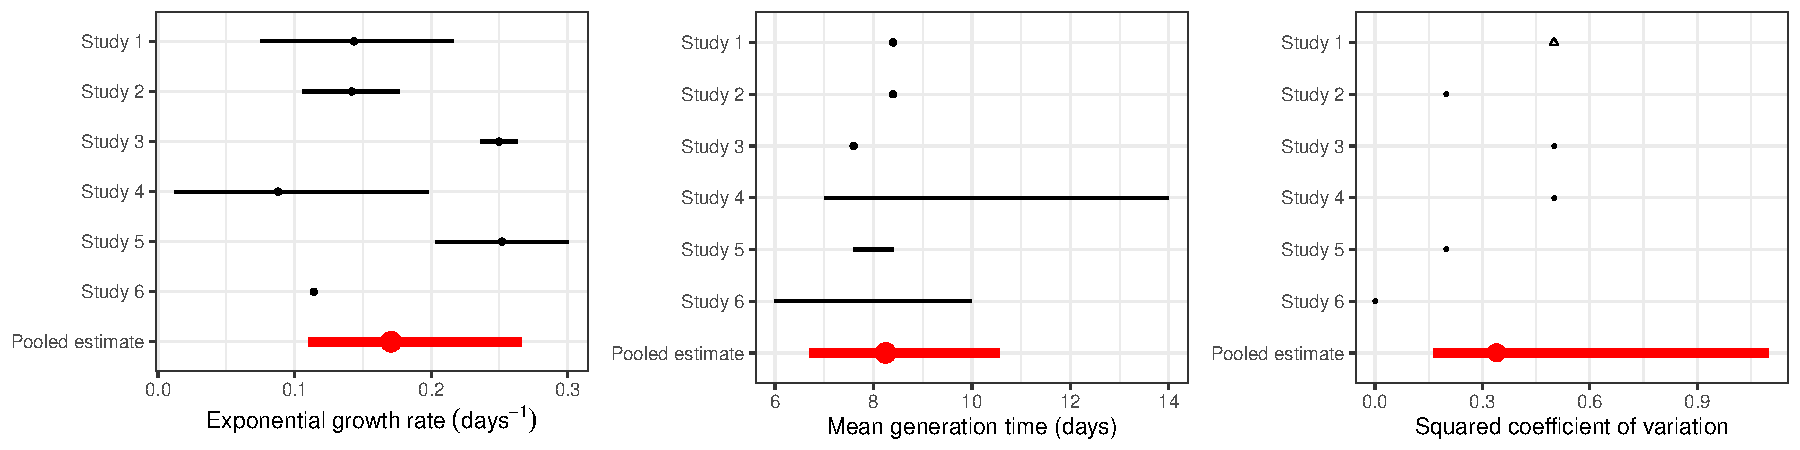
\includegraphics[width=\textwidth]{compare_assumption.pdf}
\caption{
\textbf{Comparisons of estimated and assumed parameter values with their average values calculated from the multilevel model.}
I'm a caption
}
\label{fig:assumption}
\end{figure}

\fref{assumption} compares the estimated (or assumed) values of the exponential growth rate $r$, mean generation interval $\bar G$, and the squared CV $\kappa$ of the generation-interval distribution with our pooled estimates ($\mu_r$, $\mu_G$, and $\mu_\kappa$) that we calculate from our multilevel model.
We find that there is a large uncertainty associated with the underlying parameters;
many models rely on stronger assumptions that ignore these uncertainties.
Surprisingly, no studies take into account how the variability in generation intervals (represented by $\kappa$) affects their estimates of $\mathcal R_0$, even though the assumed values range from 0 to 0.5 across different studies.

\begin{figure}[!ht]
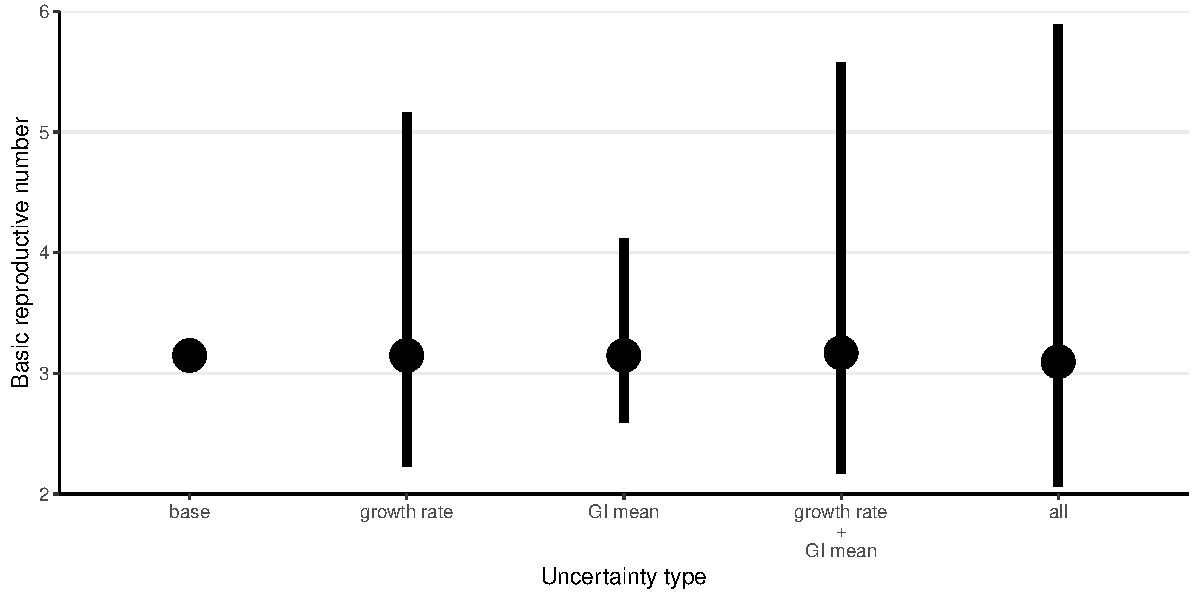
\includegraphics[width=\textwidth]{figure2.pdf}
\caption{
\textbf{Effects of $r$, $\bar G$, and $\kappa$ on the estimates of $\mathcal R_0$.}
(base): $\mathcal R_0$ estimate based on the median estimates of $\mu_r$, $\mu_G$, and $\mu_\kappa$.
(growth rate): $\mathcal R_0$ estimate based on the the full posterior distribution of $\mu_r$ while assuming median estimates of $\mu_G$ and $\mu_\kappa$.
(GI mean): $\mathcal R_0$ estimate based on the the full posterior distribution of $\mu_G$ while assuming median estimates of $\mu_r$ and $\mu_\kappa$.
(growth rate + GI mean): $\mathcal R_0$ estimate based on the the full posterior distributions of $\mu_r$ and $\mu_G$ while assuming a median estimate of $\mu_\kappa$.
(all): $\mathcal R_0$ estimate based on the the full posterior distributions of  $\mu_r$, $\mu_G$, and $\mu_\kappa$.
}
\label{fig:eff}
\end{figure}

\fref{eff} demonstrates the degree to which how the uncertainty in each parameter propogates to the uncertainties in $\mathcal R_0$.
\swp{JD: can you explain figure 2?}

Finally, we assess the validity of estimates of $\mathcal R_0$ across different studies by 
replacing the their values of $r$, $\bar G$, and $\kappa$ with our pooled estimates ($\mu_r$, $\mu_G$, and $\mu_\kappa$) one at a time and recalculating the basic reproductive number $\mathcal R_0$ (\fref{R0}).
We find that incorporating uncertainties one at a time increases the width of the confidence intervals in most cases (16 out 18).
We estimate narrower confidence intervals for Study 2 when we use our pooled estimate of the squared CV in generation time $\mu_\kappa$ to recalculate $\mathcal R_0$ because they assume a narrow generation-interval distribution ($\kappa=0$);
when lower values of $\kappa$ are used, their estimates of $\mathcal R_0$ become less sensitive to the values of $r$ and $\bar G$.
We estimate narrower confidence intervals for Study 5 when we use our pooled estimate of the mean generation time $\mu_G$ to recalculate $\mathcal R_0$ because the range of uncertainty in the mean generation time $\bar G$ they consider is much wider than ours (\fref{assumption}).

% We find that accounting for uncertainties in the estimate of $r$ (i.e., replacing the estimated $r$ values with $\mu_r$) has the largest effect on the estimates of $\mathcal R_0$ and the width of associated confidence intervals (\fref{R0}).
% For example, recalculating $\mathcal R_0$ for Study 3 by using the average $r$ values gives $\mathcal R_0 = 4.0$ (95\% CI: 2.3--10.1), which is much wider than the range they reported (2.0--3.1).
% There are two explanations for this result.
% First, even though the exponential growth rate $r$ and the mean generation time $\bar G$ have identical effects on $\mathcal R_0$ under the gamma approximation framework \eref{gamma},
% $r$ has greater overall effect on $\mathcal R_0$ because there is more uncertainty associated with our estimate of $\mu_r$ (95\% CI: 0.12--0.28 days$^{-1}$) than with $\mu_G$ (95\% CI: 6.6--10.2 days).
% Second, assuming a fixed generation time ($\kappa=0$) makes the estimate of $\mathcal R_0$ too sensitive to $r$ and $\bar G$.

\begin{figure}[t]
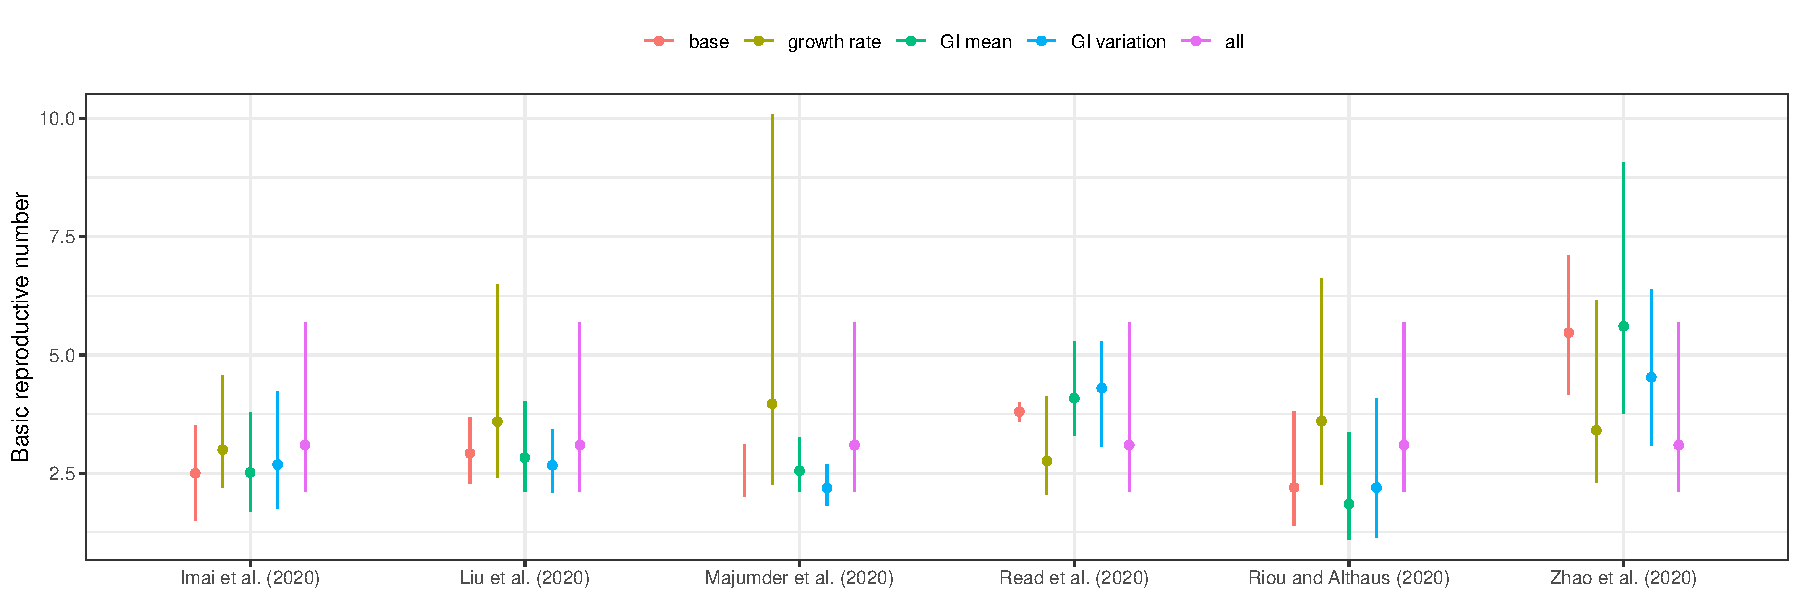
\includegraphics[width=\textwidth]{compare_R0.pdf}
\caption{
\textbf{Effect of uncertainties in underlying parameters on the estimate of the basic reproductive number.}
I'm a caption
}
\label{fig:R0}
\end{figure}

When we incorporate all uncertainties by using posterior samples for $\mu_r$, $\mu_G$, and $\mu_\kappa$ to recalculate $\mathcal R_0$ and compare it with the reported $\mathcal R_0$ estimates.
We estimate the average $\mathcal R_0$ to be 3.1 (95\% CI: 2.1--5.7).
While our pooled estimate of $\mathcal R_0$ is similar to other reported values, our calculation gives wider confidence intervals than all of them.
This result does not imply that our assumptions are too weak;
we believe that this confidence interval accurately reflects the level of uncertainties present in the information that were available when these models were fitted.
In fact, our results show that incorporating uncertainties in all parameters can give narrower confidence intervals than doing so one at a time because nonlinear effects of parameters could cancel out and give appropriately wide confidence intervals.

\section{Discussion}

Estimating the basic reproductive number $\mathcal R_0$ is crucial for predicting the course of an outbreak and planning intervention strategies.
Here, we evaluated the statistical validity of the estimates of $\mathcal R_0$ for the novel coronavirus outbreak using a novel statistical framework, based on the gamma approximation of the generation-interval distribution \citep{park2019practical}.
Our results demonstrate the importance of accounting for uncertainties associated with the underlying generation-interval distributions, especially with the amount of dispersion in the generation intervals:
assuming a narrow generation-interval distribution can make the estimate of $\mathcal R_0$ too sensitive to the estimates of the exponential growth rate $r$.

Narrow confidence intervals associated with early estimates of $\mathcal R_0$ partly depend on the statistical approches that the estimates rely on.
Of the six studies that we reviewed, two of them directly fit their models to cumulative number of confirmed cases.
Although the formula for the cumulative curve (e.g., logistic model) is much simpler and familiar to many people, 
fitting a model to cumulative number of cases can bias the parameter estimate and give overly narrow confidence intervals as it violates the ``independence of error'' assumption \citep{ma2014estimating, king2015avoidable}.
We emphasize that all models should be fitted to raw incidence data for any future analyses.



Concluding paragraph with a message?


\pagebreak

\bibliography{wuhan}

\end{document}
